% Chapter Template

\chapter{Strukturirani sažetak - Mjerenje udarnog presjeka zajedničke produkcije W bozona i para b kvarkova} % Main chapter title

\label{Chapter9} % Change X to a consecutive number; for referencing this chapter elsewhere, use \ref{ChapterX}

\lhead{Chapter 9. \emph{Strukturirani sažetak}} % Change X to a consecutive number; this is for the header on each page - perhaps a shortened title
\begin{otherlanguage}{croatian}
%----------------------------------------------------------------------------------------
%	SECTION 1
%----------------------------------------------------------------------------------------

\section{Uvod}
Standardni model fizike elementarnih čestica je teorija nastala šezdesetih i sedamdesetih godina dvadesetog stoljeća, pokušavajući odgovoriti na pitanje od čega je materija načinjena i kako interagira. Predviđanja Standardnog modela testirana su veliki put puta različitim eksperimentima, međutim nikada nisu opovrgnuta. Jedina nedostajuća karika bio je Higgsov bozon, čestica čije je postojanje portvrđeno 2012. godine, a svojstva su joj izmjerena narednih godina. Time je zaokružena slika Standardnog modela. Međutim, postoje različiti fenomeni koji ne se ne mogu opisati u okviru Standardnog modela kao što su postojanje neutrinskih oscilacija, asimetrije između materija i antimaterije, postojanje tamne materije i tamne energije. Ovi fenomeni upućuju na postojanje fizike izvan Standardnog modela. Osjetljivost pojedinog eksperimenta na opažanje takvih fenomena izravno je povezano s preciznim mjerenjem već postojećih procesa. 

Događaji u kojima je W bozon produciran zajedno s b kvarkvima u središtu je različitih teorijskih i eksperimentalnih istraživanja. Međutim, teorijska predviđanja još uvijek ne objašnjavaju dovoljno dobro  eksperimentalne rezultate zbog pojave divergencija u slučaju kada izračeni gluoni imaju jako malu energiju ili je par kvarkova kolinearan. Nadalje, precizno mjerenje W bozona produciranog s parom b kvarkova omogućava bolje razumijevanje i teorijska predviđanja u okviru perturbativne kvantne kromodinamike (pQCD) i provjere valjanosti različitih teorijskih modela korištenih u simulacijama. Ovaj proces je i pozadina za različita mjerenja u okviru Standardnog modela, uključujući mjerenja povezana s top kvarkom i Higgsovim bozonom koji se raspada u par b kvarkova. 

Tema ove teze je mjerenje udarnog presjeka za proces $pp\rightarrow W+bb+X$ koristeći podatke prikupljene CMS detektorom tijekom 2012 godine na energiji $\sqrt{s} = 8$ TeV. W bozon se raspada na elektron ili mion i odgovarajući neutrino. Prisutnost W bozona se očituje kroz postojanje izoliranog leptona visokog impulsa te nedostajuće energije koja dolazi od slabo interagirajućeg neutrina. Kvarkovi se u detektoru vide kao usmjereni mlazovi čestica te prolaze kroz posebne algoritme koji identificiraju mlazove nastale od b kvarkova.

\section{Teorijski uvod i prethodna mjerenja}

Složenost sudara protona proizlazi iz njihove unutarnje strukture. Iako je proton najvećim dijelom sastavljen od $uud$ valentnih kvarkova, ostali kvakovi koje nazivamo kvarkovima mora, te gluoni također mogu sudjelovati u sudarima. Točna predviđanja konačnih stanja u sudarima protona uvelike ovise o kombinaciji teorijskih izračuna i eksperimentalnih rezultata. Opis takvih konačnih stanja se dijeli u nekoliko stupnjeva koji se odvijaju na različitim energijskim skalama. Na najvišim energijama se odvija tvrdi proces koji rezultira produkcijom teških ili visoko-energetskih čestica. Teške čestice se potom raspadaju na lakše. Ova dva procesa opisuju se matrični elementom. Pljusak partona je idući stupanj u opisu sudara protona i označava proces u kojem su izračene lagane čestice, fotoni i gluoni, koji su često kolinearni s originalnom česticom. Zadnji stupanj je hadronizacija tijekom koje partoni formiraju hadrone čijim se raspadima produciraju stabilne čestice opažene u detektoru.
\par Prethodna mjerenja procesa koji u konačnom stanju sadrže W bozon i b kvarkove izvršena su na Tevatronu, eksperimentima CDF i D0 \cite{Aaltonen:2009qi,D0:2012qt} te na LHC-u, eksperimentima ATLAS i CMS \cite{Aad:2013vka,Chatrchyan:2013uza}. Prethodna mjerenja ne mogu se izravno uspoređivati, budući da su proučavana različita konačna stanja u različitim faznim prostorima. Međutim, usporedba sa teorijskim predviđanjima ukazuje na slaganje. 

\section{LHC}
Veliki hadronski sudarivač je ubrzivač protona smješten na švicarsko-francuskoj granici, u blizini Ženeve \cite{Evans:2008zzb}. Nalazi se u podzemnom tunelu promjera 27 km, na prosječnoj dubini od 100 m. Veliki hadnonski sudarivač je najveći u nizu akceleratora čija je zadaća postupno ubrzavanje čestica, do maksimalne energije $\sqrt{s}=$ 14 TeV. Snopovi čestica, kada dosegnu ciljanu energiju, sudaraju se na četiri mjesta gdje su izgrađeni detektori koji mjere čestice nastale u sudarima. Na dva mjesta nalaze se detektori široke namjene ATLAS (A Toroidal LHC Apparatus) \cite{Aad:2008zzm} i CMS (Compact Muon Solenoid) \cite{Chatrchyan:2008aa}.  Ovi detektori pokrivaju široki spektar tema iz fizike visokih energija, uključujući potragu za Higgsovim bozonom, supersimetričnim česticama, te detaljna mjerenja svojstava Standardnog modela. ALICE (A Large Ion Collider Experiment) detektor proučava kvarkovsko-gluonsku plazmu u sudarima iona olova \cite{Aamodt:2008zz}. LHCb (LHC Beauty) je usmjeren na pručavanje B fizike kroz raspade B mezona \cite{Alves:2008zz}. LHC je modularni ubrzivač sastavljen od oko 10000 različitih supravodljivih magneta koji fokusiraju i usmjeravaju snop čestica.
\par Snopovi se ubrizgavaju u LHC u obliku paketa protona te se ubrzavaju pomoću radiofrekventnih komora (RF). Tijekom 2012. godine, prosječan broj sudara je bio oko 21 unutar jednog sudara paketa protona. Broj sudara po jedinici vremena se naziva luminozitet, a ukupan broj sudara se u nekom vremenskom periodu se naziva integrirani luminozitet. Tijekom 2012. godine ukupno je prikupljeno više od 24 fb$^{-1}$ inegriranog luminoziteta. 

 
\section{CMS detektor}
Kompaktni mionski solenoid (CMS) izgrađen je oko jedne od četiri točaka interakcije na velikom hadronskom sudarivaču. Detektor je slojevitog cilindričnog dizajna, hermetički zatvoren i gotovo potpuno pokriva cijeli prostorni kut oko točke interakcije. CMS detektor koristi desni koordinatni sustav s ishodištem u središtu detektora. $z$ os je postavljena duž smjera snopa, $x$ os je usmjerena prema središtu prstena, a $y$ os je okomita na njih. Detektor je podijeljen na centralni dio ($barrel$) koji se proteže do $\eta \approx \pm 1.5$, te bočne dijelove ($endcaps$). Unutar CMS-a nalazi se solenoid koji generira polje od 3.8 T u unutarnjem volumenu i oko 2 T izvan.  Unutar solenoida nalaze se detektor tragova i kalorimetri, a izvan mionske komore. Jako magnetsko polje zakreće putanje nabijenih čestica nastalih u sudarima i omogučava mjerenje njihovog impulsa. 
\par U samom središtu detektora, oko točke interakcije, smješten je silicijski piksel detektor. Sastoji se od tri sloja u središnjem dijelu i dva diska sa svake strane i sadrži oko 66 milijuna piksela. Oko njega nalazi se silicijski $strip$ detektor, koji se sastoji od niza žica. U žicama se prolaskom nabijene čestice inducira naboj koji se potom dovodi do silicijskih detektora. 
\par Elektromagnetski kalorimetar (ECAL) izgrađen je od olovnog volframata, kristala velike gustoće i malog Moliereovog radijusa, što rezultira kratkim i uskim pljuskovima prilikom upada fotona ili elektrona. Hadronski kalorimetar (HCAL) sastoji se od slojeva mjedenih absorbera i plastičnih scintilatora u središnjem dijelu, te čeličnih absorbera i kvarcnih scintilatora u bočnim dijelovima. Svrha hadronskog kalorimetra je zastavljanje hadronskih snopova, što se događa u absorberima, a rezultirajući pljusak čestica se detektira scintilatorima. 
\par Mionske komore sastoje se od nekoliko vrsta detektora punjenih plinom. Driftne komore smještene su u središnjem dijelu i napunjene su plinom koji se ionizira prolaskom čestice. Katodne trakaste komore nalaze se u bočnim dijelovima te funkcioniraju na isti način kao i driftne komore, ali su dodatno isprepletene velikim brojem žica za prikupljanje naboja. Komore s otpornim pločama sastoje se od paralelnih ploča velike otpornosti između kojih je plin. U slučaju prolaska čestice dolazi do ionizacije plina i stvaranja pljuska elektrona. Ove detektore karakterizira visoka vremenska razlučivost, te su pogodni za korištenje kao dio sustava za okidanje. 
\par Protoni u LHC-u se sudaraju frekvencijom od 40 MHz i generaju veliku količinu podataka koju nije moguće pohraniti. Uzimajući u obzir da su udarni presjeci za zanimljive fizikalne procese redove veličina manji od udarnog presjeka za sudar protona, potrebno je konstruirati sustav okidača koji će zapisivati samo zanimljive događaje. Ovaj sustav je dizajniran na dvije razine. Prva razina koristi posebnu elektroniku i pomoću jednostavnih zahtjeva na svaki događaj, uspijeva unutar 3 $\mu$s smanjiti broj događaja s 40 MHz na oko 100 kHz. Iduća razina se naziva \textit{High Level Trigger} (HLT), čija je zadaća smanjiti broj sudara na oko 100 u sekundi.       

\section{Rekonstrukcija fizikalnih objekata}
\par Elektoni u detektoru ostavljaju trag u detektoru tragova i deponiraju energiju u elektromagnetskom kalorimetru. Elektron prolaskom kroz materijal može emitirati i tzv. zakočno zračenje, odnosno fotone koji također deponiraju energiju u elektromagnetskom kalorimetru. Svi energetski depoziti od jednog elektrona formiraju tzv. $supercluster$ koji se potom kombinira s tragom u detektoru tragova koristeći GSM (\textit{Gaussian Sum Filter}) algoritam \cite{CMS:2010bta,2005JPhG31N9A}.
\par Mione karakterizira trag u detektoru tragova i signali u mionskim komorama. Rekonstrukcija kreće od mionskih komora gdje se prilagodbama iz signala rekonstruira trag (tzv. \textit{stanalone muon}). Zatim se izgrađuje globalni mion kombiniranjem traga iz detektora tragova i traga iz mionskih komora \cite{2012JInst7P0002T,Fruhwirth1987444}.   
\par Mlazovi su usmjerena grupa hadrona koja nastaje kao rezultat fragmentacije i hadronizacije kvarkova. Detektirani hadroni se kombiniraju u mlaz posebnim algoritmima, čime se pokušavaju saznati informacije o početnom partonu. Najpopularniji takav algoritam je anti$-k_T$ algoritam koji na osnovu udaljenosti čestica i njihovih impulsa grupira čestice unutar unaprijed definiranog konusa oko čestice najvišeg impulsa \cite{Cacciari:2008gp}. Proces je iterativan i nastavlja se sve dok svi hadroni ne budu pridruženi nekom mlazu. 
\par Mlazovi iz b kvarkova se identificiraju pomoću posebnih algoritama \cite{Chatrchyan:2012jua}. Ti algoritmi koriste karakteristična svojstva b kvarkova kao što su njihova masa i dugo vrijeme života za formiranje jedinstvene varijable koja definira koliko je neki mlaz nalik na mlaz nastao iz b kvarka. Algoritam korišten u ovoj tezi je CSV (\textit{Combined secondary vertex}) koji traga za sekundarnim točkama interakcije koje su odmaknute od mjesta sudara i gleda tragove čestica iz tog mjesta sudara.
\par Nedostajuća transverzalna energija je neravnoteža u transverzalnom impulsu svih detektiranih čestica i određuje se kao:
\begin{equation}
E_T^{miss}= |-\sum_{i} \vec{p}_i|.
\end{equation}
Budući da je trasverzalni impuls očuvan, nedostajuća energija mjeri impuls kojeg odnose nevidljive čestice. Određivanje nedostajuće energije je ovisno o rezoluciji detektora, ograničenoj pokrivenosti prostornog kuta, pogrešnom interpretacijom detektiranog signala ili kozmičkim zrakama. Ove pojave mogu umjetno povećati iznos nedostajuće energije što treba uzeti u obzir \cite{Chatrchyan:2011tn}.  

\section{Selekcija događaja i navažnije pozadine}
 
U tezi su predstavljeni rezultati mjerenja udarnog presjeka za produkciju W bozona zajedno s parom mlazova nastalih iz b kvarka u sudarima protona na energiji $\sqrt{s}=$ 8 TeV. Podaci su prikupljeni 2012. godine CMS detektorom i odgovaraju integriranom luminozitetu od 19.8 fb$^{-1}$. Za simuliranje signala i pozadine korišteni su generatori Madgraph \cite{Alwall:2011uj}, Powheg \cite{Oleari:2010nx} i Pythia \cite{Sjostrand:2006za}. 
\par Zbog boljeg slaganja podataka i simulacija, na simulacije se primjenjuje niz korekcija:
\begin{itemize}
\item Korekcije zbog različitog broja primarnih interakcija. Budući da su simulirani uzorci često generirani prije nego što su uvjeti tijekom prikupljanja podataka poznati, kao što je trenutni luminozitet, potrebno je korigirati simulirane događaje. Korekcija se provodi pridavanjem težine svakom simuliranom događaju tako da raspodjela broja primarnih interakcija u događaju izgleda jednako u podacima i simulacijama \cite{CMS:2013wea}.
\item Efikasnost identifikacije, izolacije i okidača za leptone. Efikasnosti su određene iz podataka korištenjem tzv. \textit{Tag-and-probe} metode, ovisne su o transverzalnom impulsu i pseudorapiditetu te se primjenjuju kao težine za svaki simulirani događaj.
\item Efikasnost algoritma za određivanje b mlazova. Budući da je teško točno modelirati sve parametre koji ulaze u algoritam za određivanje b mlazova, potrebno je korigirati simulirane događaje za omjer efikasnosti algoritma u podacima i simulacijama \cite{CMS:2013vea}.
\end{itemize}
\par Događaji korišteni za mjerenje udarnog presjeka moraju sadržavati W bozon koji se raspada na mion ili elektron, te značajnu količinu nedostajuće energije koja ukazuje na postojanje neutrina. Rekonstruirani mlazovi čestica trebaju zadovoljavati kriterije za b mlazove. Svi kriteriji za selekciju događaja sabrani su ovdje:
\begin{itemize}
\item Jedan mion ili elektron s $p_T>$ 30 GeV i $|\eta|<$2.1  i izolacijskom varijablom $I_{rel}^{PF}<0.12\ (0.10)$ za mione (elektrone),
\item Točno dva mlaza s $p_T>$ 25 GeV i $|\eta|<$2.4 i konusom između mlaza i leptona većim od 0.5,
\item Događaji koji sadrže više od dva mlaza s $p_T>$ 25 GeV i $|\eta|<$2.4 su odbačeni,
\item Događaji koji sadrže dodatni lepton s $p_T>$ 10 GeV i $|\eta|<$2.1 su odbačeni,
\item Oba mlaza moraju imati disktiminantu za određivanje b-mlazova veću od 0.898,
\item Iznos transverzalne mase mora biti veći od 45 GeV.
\end{itemize}  

Najvažnije pozadine uključuju procese s t kvarkovima, Z i W bozone producirane zajedno s mlazovima, dvobozonske događaje te QCD događaje. Pozadine s t kvarkovima su reducirane zahtjevima za točno jednim leptonom i dva mlaza, međutim nakon toga zahjeva, doprinos od tih procesa u konačnom uzorku je oko 60$\%$. Zbog toga je konstruirano posebno kontrolno područje dominirano doprinosom procesa s t kvarkovima u konačnom stanju s ciljem provjere normalizacije tih procesa. Kontrolno područje je dobiveno zahtjevom za više od dva mlaza u konačnom stanju. Uočeno je da je razlika između podataka i simulacija oko 12$\%$ što je uzeto u obzit prilikom određivanja broja događaja signala. 
\par Događaji koji sadrže Z bozon i mlazove u konačnom stanju mogu proći selekciju ako jedan lepton nije dobro rekonstruiran, čime se umjetno stvara nedostajuća energija. Procesi s W bozonom i mlazovima nastalim od lakih kvarkova u konačnom stanju reducirani su na zanemarive vrijednosti postavljanjem zahtjeva na diskriminatornu varijablu b tagging algoritma. Dvobozonski procesi u kojima nastaju W i Z bozon koji se potom raspada na par b kvarkova čine ireducibilnu pozadinu. QCD procesi u konačnom stanju sadrže lepton koji uspjeva proći konačnu selekciju, ali nije nastao raspadom W bozona. Ova pozadina se određuje direktno iz podataka. Oblik raspodjele je određen invertiranjem izolacije na lepton i oduzimanjem MC doprinosa od podataka. Normalizacija raspodjele određuje se u području niskih vrijednosti transverzne mase $M_T<$ 30 GeV.

\section{Rezultati}

Udarni presjek za proces pp$\rightarrow$W+bb+$X$ mjeren je odvojeno u elektronskom i mionskom kanalu i određen je izrazom:
\begin{equation}
\sigma = \frac{N_{sig}}{A\times \epsilon \cdot \mathcal{L}}
\label{equ:xsec_hr}
\end{equation}
gdje je $N_{sig}$ ukupni broj događaja signala koji je određen prilagodbom. $A\times \epsilon$ definira aktivno područje i efikasnost detektora, a $\mathcal{L}$ integrirani luminozitet. 
Aktivno područje i efikasnost detektora definirano je kao:
\begin{equation}
A\times \epsilon=\frac{\mathrm{broj\ izabranih\ Wbb\ događaja}}{\mathrm{broj\ generiranih\ Wbb\ događaja}}
\end{equation}
Ova se vrijednost određuje iz simulacija za svaki kanal posebno. Rezultat je naveden u tablici \ref{tab:AE_hr}.
\begin{table}[!htb]
\begin{center}
   \begin{tabular} {r c} \hline \hline
        Channel         & A$\times \epsilon$ \\
        \hline
        Mionski kanal         & 9.14 $\pm$ 0.18 $\%$ \\
        Elektronski kanal     & 7.66 $\pm$ 0.17 $\%$ \\
        \hline\hline
   \end{tabular}
\caption{Rezultati određivanja A$\times \epsilon$ za mionski i elektronski kanal.}
\label{tab:AE_hr}
\end{center}
\end{table}
Broj događaja signala određen je prilagodbom distribucije transverzne mase koristeći metodu najveće vjerodostojnosti (\textit{maximum likelihood fit}). Prilagodba je izvedena istovremeno u signalnom području i u prethodno opisanom kontrolnom području koristeći distribucije prikazane na slici \ref{fig:mt_hr}. Sistematski efekti su također uzeti u obzir na način da su za svaki doprinos i za svaku pozadinu producirane dvije dodatne distribucijem koje odgovaraju pomaku od jedne standardne devijacije gore i dolje u odnosu na nominalnu vrijednost. Promatrani izvori sistematskih neodređenosti su:
\begin{itemize}
\item Mjerenje energije mlazova,
\item Rezulucija mlazova,
\item Efikasnost određivanja b mlazova,
\item Mjerenje energije leptona,
\item Efikasnost okidača te identifikacije i izolacije leptona,
\item Nedostajuća energija od mlazova niskih energija,
\item Normalizacije simuliranih uzoraka,
\item Mjerenje luminoziteta.
\end{itemize}
\begin{figure}[htbp]
	\centering
		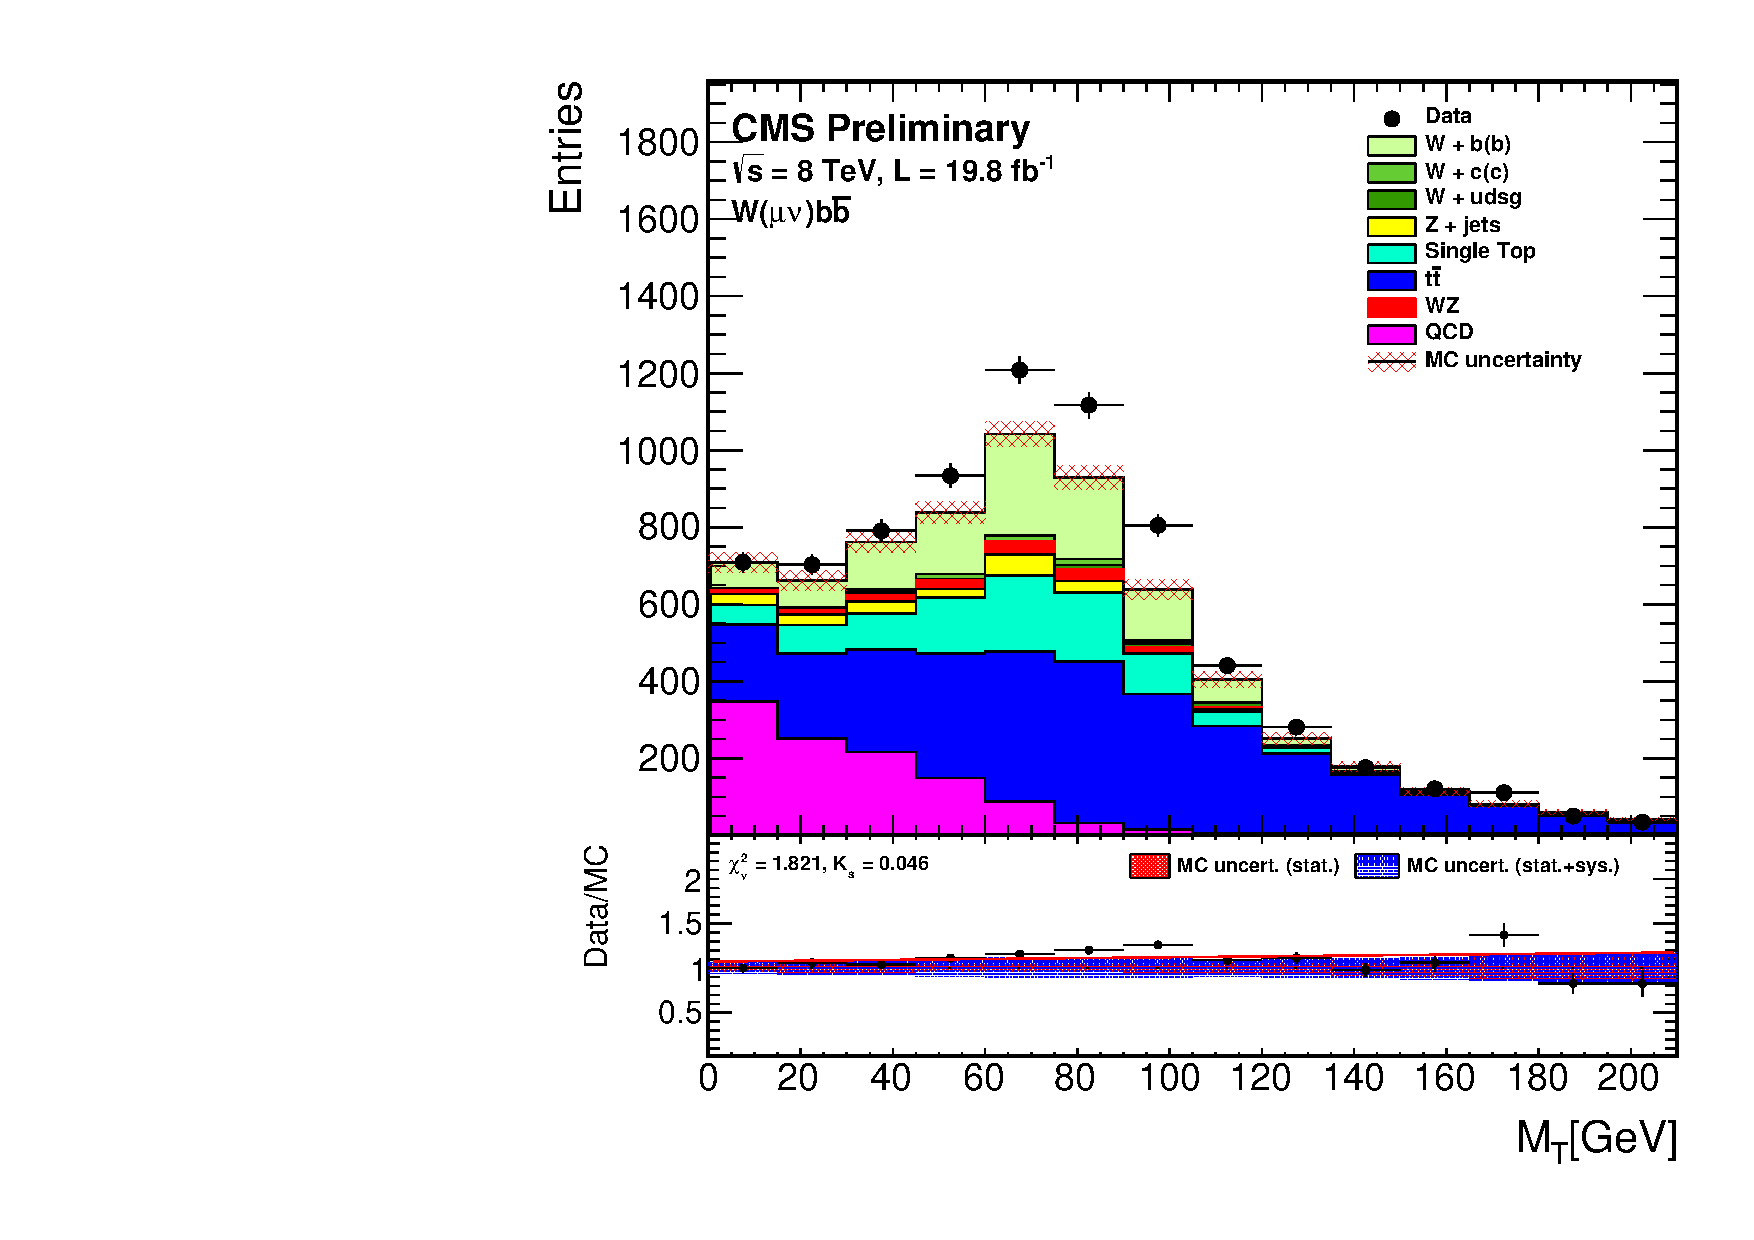
\includegraphics[width=0.48\textwidth]{Figures/Results/Muon/prefit/Wbb_GetVMt_doQCD1.pdf}
		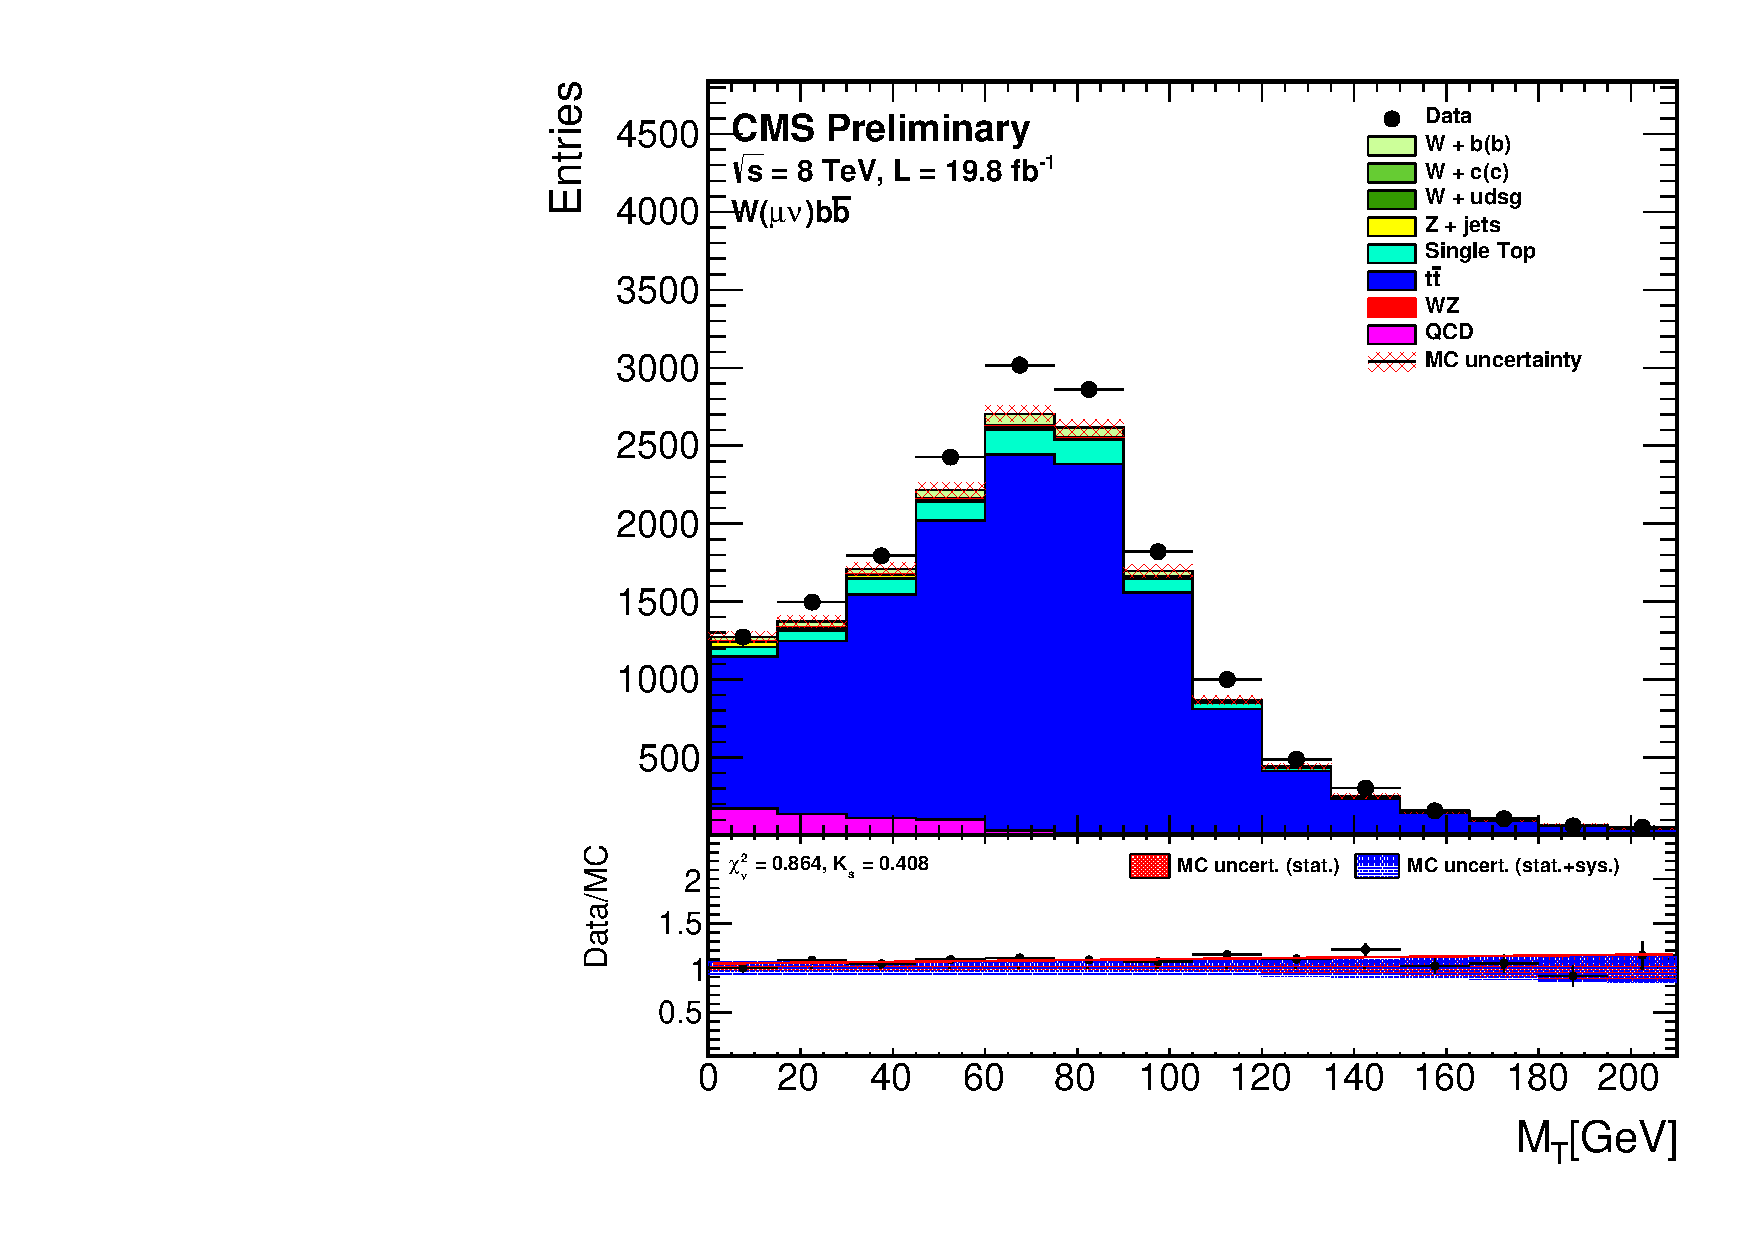
\includegraphics[width=0.48\textwidth]{Figures/Results/Muon/prefit/TT_GetVMt_doQCD1.pdf}
		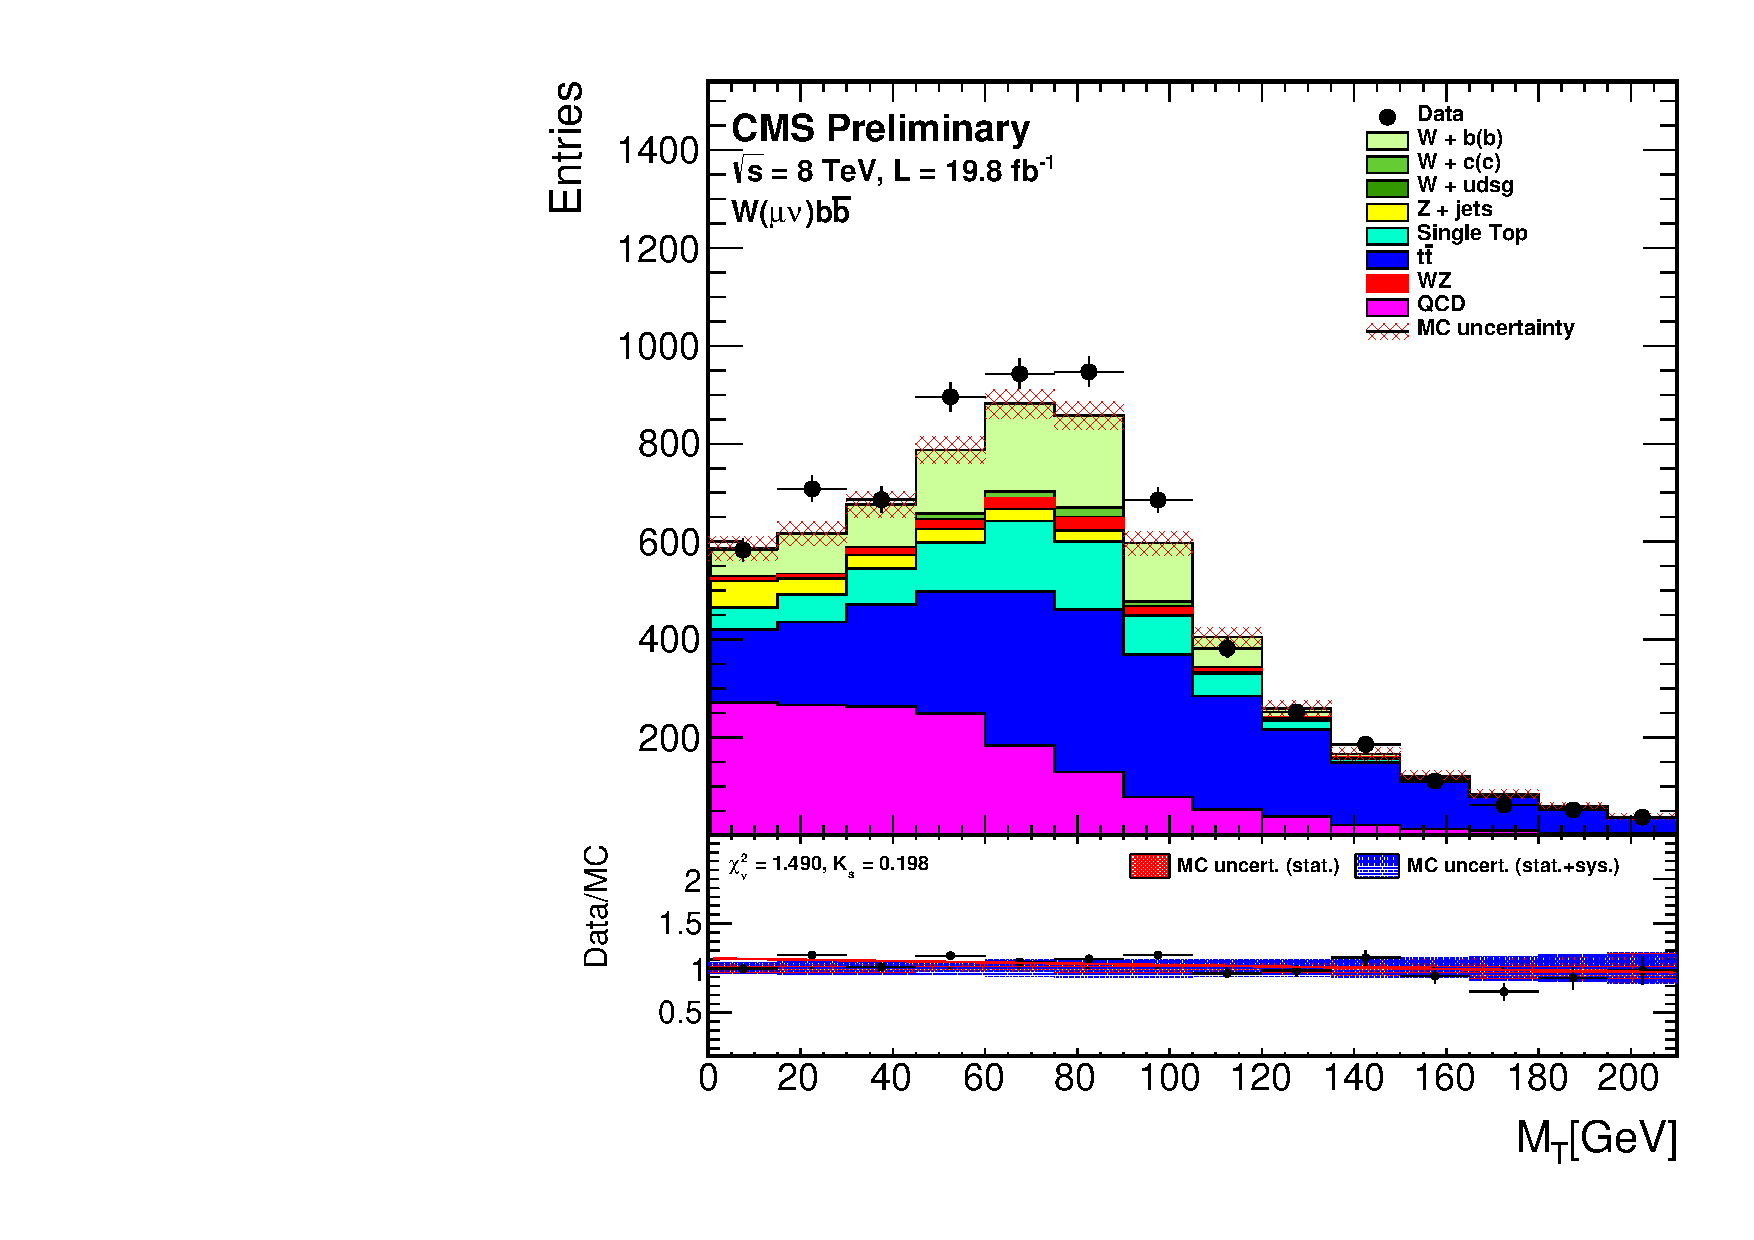
\includegraphics[width=0.48\textwidth]{Figures/Results/Electron/prefit/Wbb_GetVMt_doQCD1.pdf}
		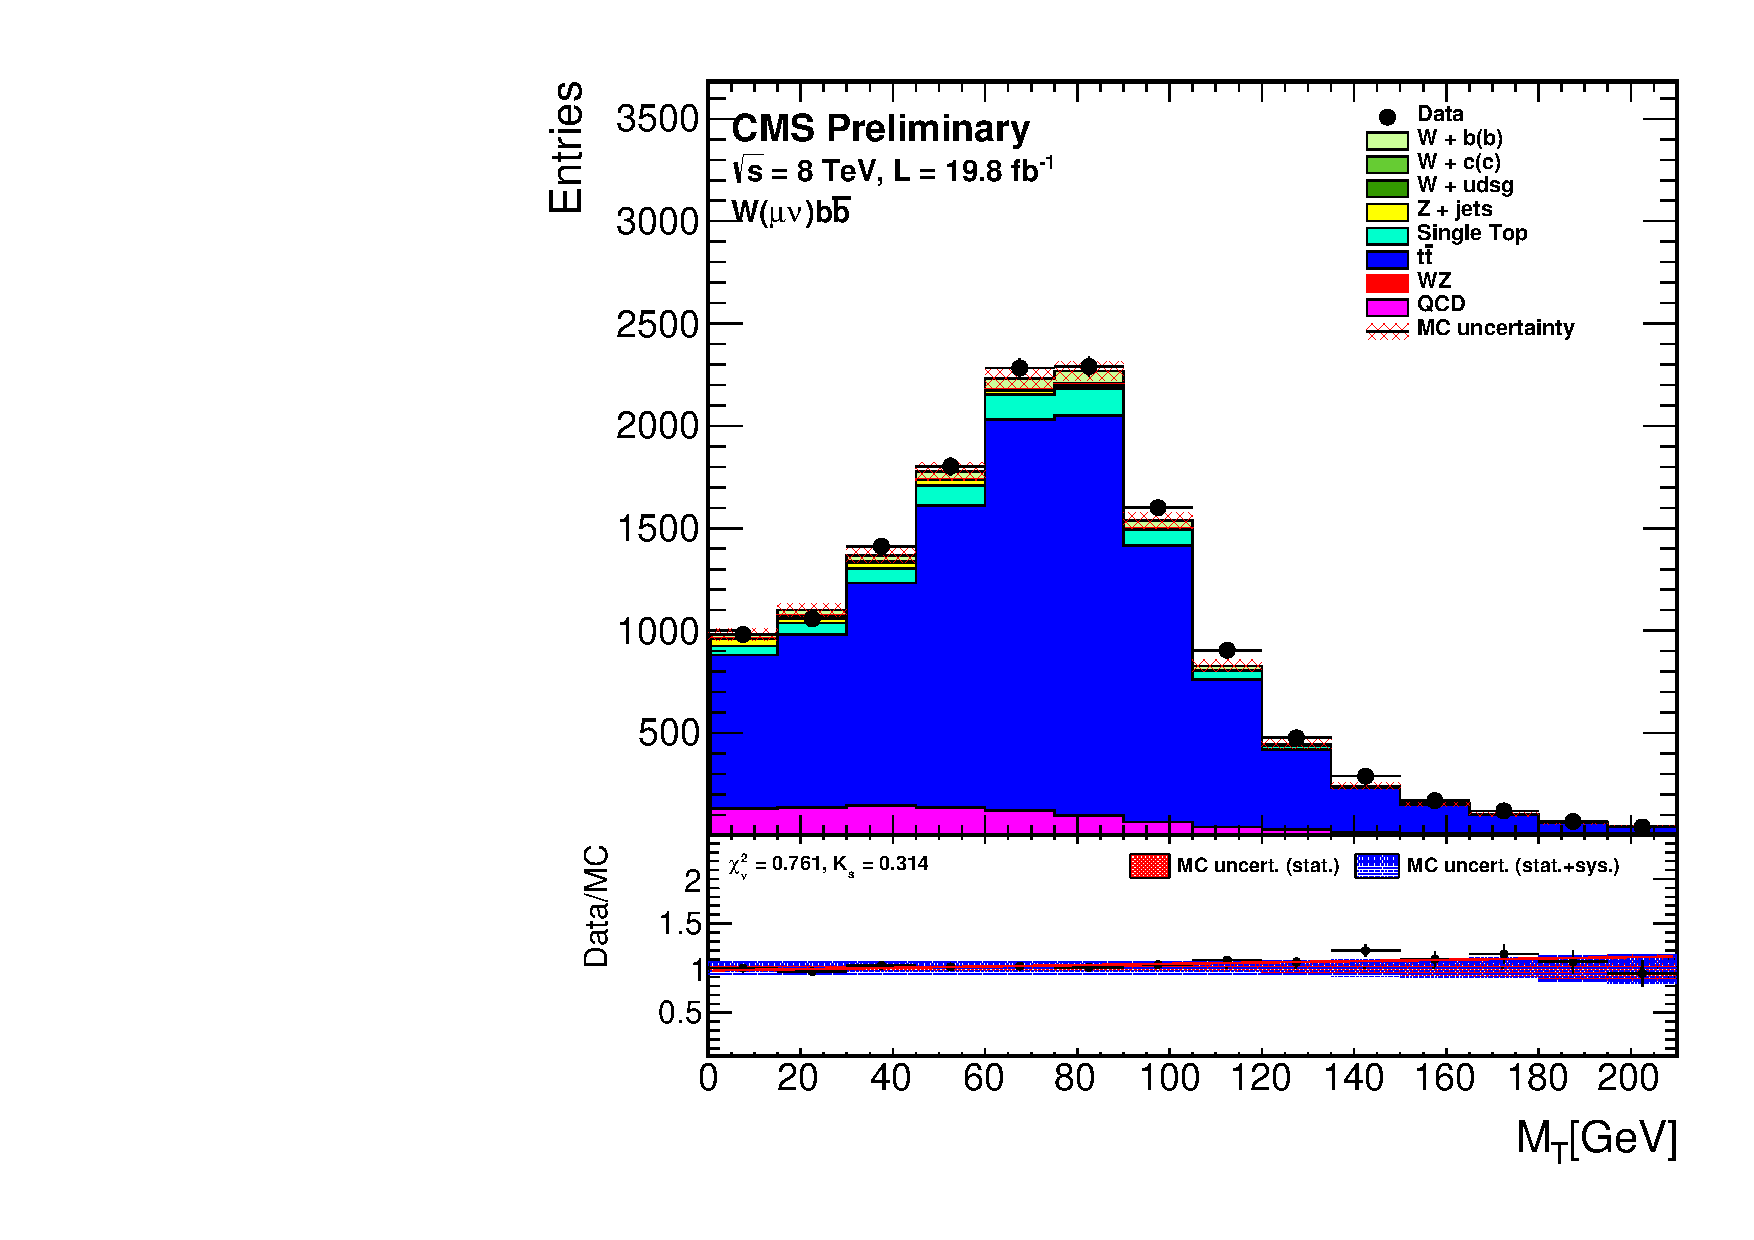
\includegraphics[width=0.48\textwidth]{Figures/Results/Electron/prefit/TT_GetVMt_doQCD1.pdf}
		%\rule{35em}{0.5pt}
	\caption[Transverse mass distributions]{Distribucije transverzne mase za mionski (\textit{gore}) i elektronski (\textit{dolje}) za signalno područje i kontrolno područje dominitanu top kvark pozadinom.}
	\label{fig:mt_hr}
\end{figure}

U konačnoj prilagodbi svi doprinosi variraju unutar neodređenosti osim signala koji je slobodan. Konačni rezultat, iskazan kao omjer mjerenog udarnog presjeka i teorijskog predviđanja (\textit{signal strength}), označava se sa $\mu$ i iznosi:
\begin{align*}
\mu_{mu} &= 1.37 \pm 0.07\mathrm{(stat.)} \pm 0.20 \mathrm{(syst.)}\\\
\mu_{ele} &= 1.67 \pm 0.08\mathrm{(stat.)} \pm 0.27\mathrm{(syst.)}
\end{align*}
Korištenjem relacije \ref{equ:xsec_hr} može se sada odrediti udarni presjek. Broj događaja signala je definiran kao broj događaja prije prilagodbe pomnožen s $\mu$. Aktivni dio detektora i efikasnost se uzimaju iz tablice $\ref{tab:AE_hr}$, a integrirani luminozitet iznosi 19.8 fb$^{-1}$. Dobiveni vrijednost udarnog presjeka je:
\begin{align*}
\sigma(pp\rightarrow W+bb)\times \mathcal{B}(W\rightarrow \mu\nu) = 0.66 \pm 0.03(\mathrm{stat.}) \pm 0.10(\mathrm{syst.})\\
\sigma(pp\rightarrow W+bb)\times \mathcal{B}(W\rightarrow e\nu) = 0.78 \pm 0.04(\mathrm{stat.}) \pm 0.13(\mathrm{syst.})
\end{align*} 
Navedeni rezultati uključuju sve prethodno navedene sistematske neodređenosti. Međutim, u obzir nisu uključene sistematske neodređenosti na određivanje aktivnog dijela detektora i efikasnosti prilikom različitog odabira partonske distribucijske funkcije i varijacije renormalizacijske i faktorizacijske skale.
\par Teorijsko predviđanje određeno je MCFM paketom na NLO preciznost s faktorizacijskom i renormalizacijskom skalom postavljenom na masu W bozona. Uzimajući u obzir i doprinos događaja u kojima su se sudarila po dva partona iz svakog protona (\textit{Double parton scattering - DPS}) \cite{Chatrchyan:2013xxa}, udarni presjek tada iznosi:
\begin{equation*}
\sigma_{TH}(pp\rightarrow W+bb)\times \mathcal{B}(W\rightarrow l\nu) = 0.55 \pm 0.03 \mathrm{(theor.)} \pm 0.02 \mathrm{(DPS)} \mathrm{\ pb}.
\end{equation*}

 

\section{Zaključak}

Ova teza predstavlje rezultate mjerenja udarnog presjeka za produkciju W bozona zajedno s parom mlazova nastalih iz b kvarka u sudarima protona na energiji $\sqrt{s}=$ 8 TeV. Podaci su prikupljeni 2012. godine CMS detektorom i odgovaraju integriranom luminozitetu od 19.8 fb$^{-1}$. Udarni presjek je mjeren posebno u elektronskom i mionskom kanalu, a dva su rezultata kompatibilna unutar neodređenosti. Teorijsko predviđanje za ovaj proces izračunato je pomoću MCFM paketa. Mjerena vrijednost je za jednu standardnu devijaciju viša od predviđene teorijske vrijednosti. Neodređenost mjerenja udarnog presjeka je dominirana sistematskim pogreškama, prvenstveno neodređenošću identifikacije b mlazova. Smanjanje ovih efekata bi omogućilo testiranje predviđanja perturbativne kromodinamike. Daljnja istraživanja ovog i sličnih procesa uključuju i mjerenje diferencijalnog udarnog predjeka u ovisnosti o npr. transverzalnom impulsu vodećeg b mlaza što bi dovelo do unapređenja torijskih modela. Nadalje, mogu se proučavati i stanja u kojim su dva B hadrona u istom mlazu što bi dovelo do boljeg razumijevanja kolinearnih konačnih stanja. 

\end{otherlanguage}
